\chapter{Implementation}

\section{Hosting and Server Management}
The hosting solution we decided on is a Virtual Private Server (VPS) running on Linux provided by company Váš hosting.
It comes ready with a lot of tools to manage the server, is fully prepared for hosting,
is accessible via SSH and has a web-based control panel for managing the server.

After installing the .NET 8 runtime the process of running a .NET application was as simple as transfering the program via SFTP
and inputting 'dotnet Afantazie.dll' into the terminal.
Deploying the frontend required only copying the files to the necessary directory in the server filesystem.
DNS and SSL certificates got set-up in a mouse click in provided server-management.

The greatest challenge when hosting the application came with setting up reverse-proxy server (although that was mostly due to our inexperience with the technology).
Two provided reverse proxy server technologies were the default Apache and NginX.
After a short research through forums we decided to make the switch to NginX as it is more modern alternative to Apache and can have performance benefits. xxx{(cit needed.)}
If needed we could always switch back Apache without much hassle.

The provided template for the NginX configuration was a good starting point but in order to make the
application functional we had to make a few additions to the afantazie.cz.conf file:
\begin{itemize}
    \item Reroute the api requests to the backend
    \item Set up redirection from http to https
    \item Force the server to always provide new version of meta.json file used for cache busting \xxx{more below}
\end{itemize}

With that the server was set up to host the database, backend and frontend.

\section{React Chat application}
As a warmup before graph rendering we built a small chat application in React.
We provided basic functionalities for authX/Y, real-time chat and a few pages:
\begin{itemize}
    \item Home page
    \item Login page
    \item Registration page
    \item Chat page
    \item About page
\end{itemize}

\subsection{Backend}
The backend of the chat application is an ASP.NET application written in C\#.
We decided to develop architectural design early on and it paid off as developing later features was much easier. 
The initial architectural blueprint remained mostly unchanged right until the end of the project.

The architecture \xxx{is in figure:}


\subsection{Frontend}
The frontend of the application is a React web application written in Typescript. 

\subsection{Server-Client communication}
websockets then signalR

\section{Small graph vizualization}
...
...
...
In the end we had an application with comparable graph view to obsidian. \ref{Selfie_for_bc_p.png} \xxx{todo - simple arrows}

In figure \ref{obr:afantazie_cithep_3k} you can see again the first 3000 nodes of the citHep dataset now visiaulised using Aphantasia.
With this many nodes on screen the application lagged a lot. Although it remained somewhat usable.

\begin{figure}[p]\centering
    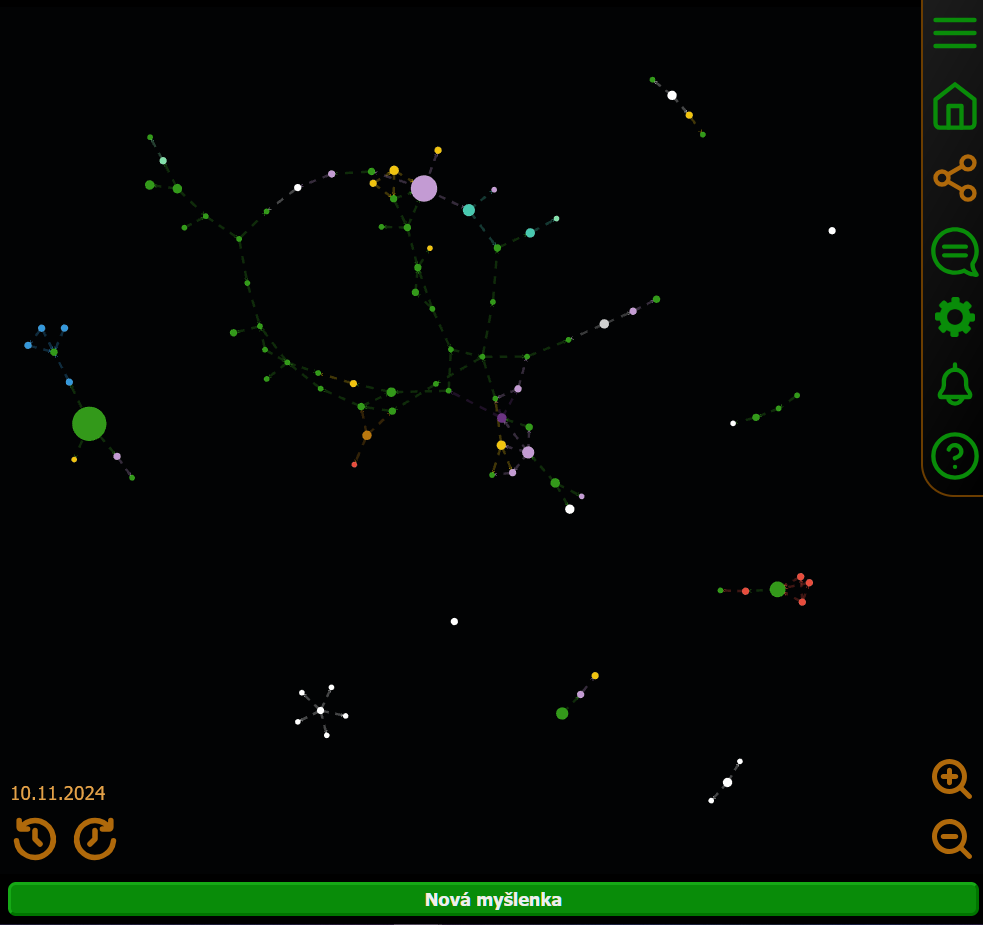
\includegraphics[width=140mm, height=140mm]{img/Selfie_for_bc_p.png}
    \caption{Aphantasia web application}
    \label{obr:afantazie_selfie}
\end{figure}

\begin{figure}[p]\centering
    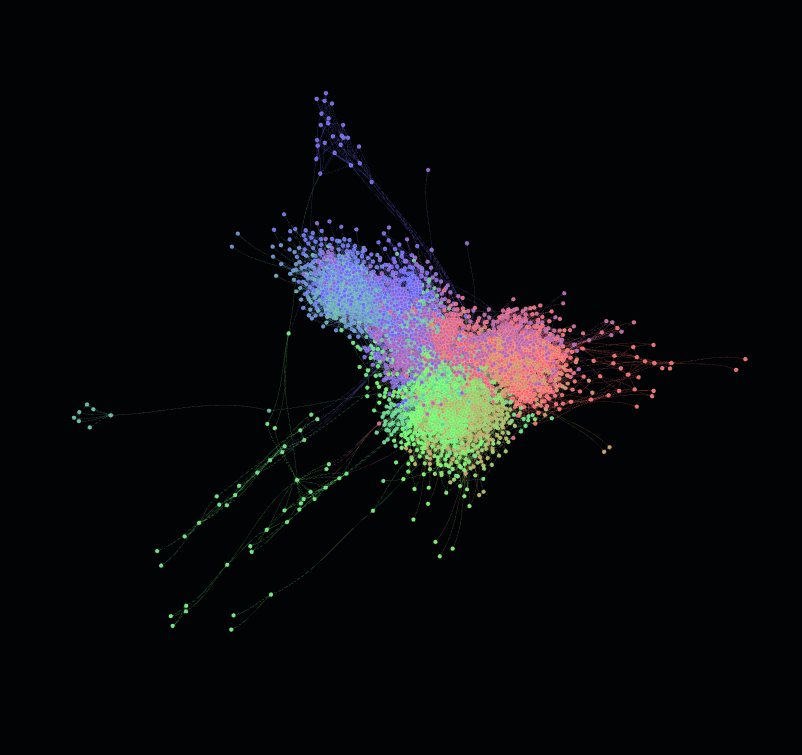
\includegraphics[width=140mm, height=140mm]{img/Afantazie_cithep_3000.png}
    \caption{The first 3000 nodes of the CitHep dataset visualized in Aphantasia (before big graph implementation)}
    \label{obr:afantazie_cithep_3k}
\end{figure}
  

\section{Big graph visualization}
We had to implement time slider and that provided a suprisingly nice way of handling big graphs.

\section{Force directed layout implementation}
pull, push, gravity, lots of parameters and tweaking, jitter, performance, overlap, graph walk optimization

\subsection{Dynamic loading}
At the beginning of the development we used one endpoint for all the data. That worked until around 500 thoughts afther which the loading time became quite noticable. 

The obvious solution was to load only a subset of the data at a time. We implemented this in several ways:
\begin{itemize}
    \item \textbf{Temporal API endpoints} - Client requests new subset of nodes in a form of "beforeId / afterId / aroundId".
    Thanks to ascending ID increment approach translates to chronological order of the nodes.
    When time window exceeds the currently loaded data it gets updated with missing nodes from the relative past or future.
    \item \textbf{Neighborhood API endpoints} - Breadth-first search starting in given node up to given depth. is used to implement graph walk.
    \item \textbf{\xxx{Filters}} - User can filter the nodes by author.
\end{itemize}